% =====================================================================
% O CÁLCULO AUSENTE — versão para submissão à
% Revista de Educação Matemática (REMat/SBEM-SP)
%
% IMPORTANTE: arquivo ANONIMIZADO para avaliação por pares duplo-cega.
% Identificação dos autores (nomes, ORCID, Lattes, e-mails) consta
% APENAS na folha de rosto separada e nos metadados do sistema OJS,
% conforme as Orientações de Submissão da REMat.
%
% Normas atendidas: Times New Roman 12; espaço 1,5; recuo 1,25 cm;
% margens sup./inf. 3,0 cm e esq./dir. 2,5 cm; A4; ABNT NBR 10520:2023
% (autor-data); quadros/tabelas sem fios verticais, título acima,
% fonte abaixo; resumos em PT/EN/ES.
%
% Compilação: tectonic calculo-remat-submissao.tex
%           (ou: pdflatex 2x, se preferir o motor tradicional)
% =====================================================================

\documentclass[12pt,a4paper,oneside]{article}

\usepackage[T1]{fontenc}
\usepackage[utf8]{inputenc}
\usepackage[brazilian]{babel}
\usepackage{newtxtext}
\usepackage{newtxmath}
\usepackage[a4paper,top=3cm,bottom=3cm,left=3cm,right=2.5cm]{geometry}
\usepackage{setspace}
\usepackage{indentfirst}
\usepackage{titlesec}
\usepackage{caption}
\usepackage{booktabs}
\usepackage{array}
\usepackage{graphicx}
\usepackage{float}
\usepackage[hidelinks,breaklinks=true]{hyperref}
\usepackage{url}
\usepackage{xurl}

\graphicspath{{figures-calculo/}}

\onehalfspacing
\setlength{\parindent}{1.25cm}
\setlength{\parskip}{0pt}
\setlength{\emergencystretch}{2em}

% --- Seções primárias: TNR 12, negrito, MAIÚSCULAS, justificado ------
\titleformat{\section}{\normalfont\normalsize\bfseries}{\thesection}{0.6em}{\MakeUppercase}
\titleformat{\subsection}{\normalfont\normalsize\bfseries}{\thesubsection}{0.6em}{}
\titleformat{\subsubsection}{\normalfont\normalsize\itshape}{\thesubsubsection}{0.6em}{}
\titlespacing*{\section}{0pt}{14pt}{6pt}
\titlespacing*{\subsection}{0pt}{10pt}{4pt}
\titlespacing*{\subsubsection}{0pt}{8pt}{3pt}

% --- Quadros/Tabelas: título acima, fonte size 10, sem fios verticais
\captionsetup[table]{labelfont=bf,name=Quadro,labelsep=endash,
                     position=above,justification=centering,font=normalsize,skip=4pt}
\captionsetup[figure]{labelfont=bf,name=Figura,labelsep=endash,
                      position=below,justification=centering,font=small,skip=4pt}

% comando para a linha "Fonte:" sob quadros/tabelas
\newcommand{\fonte}[1]{\par\vspace{1pt}{\footnotesize\noindent\hspace*{0pt}Fonte: #1}}

\begin{document}

% =====================================================================
% TÍTULO + RESUMOS  (sem identificação de autoria — avaliação cega)
% =====================================================================
% Título em Português (idioma principal, tamanho 14, máximo 15 palavras)
\begin{center}
{\fontsize{14}{17}\selectfont\bfseries O cálculo ausente: duzentos anos de
currículo e uma comparação internacional no ensino médio}
\end{center}

\vspace{4pt}

% ---------- RESUMO (PT) ----------
\noindent\textbf{RESUMO}\\[2pt]
{\setstretch{1.0}\small\noindent
Este artigo conduz uma revisão documental comparada dos currículos
oficiais de matemática do ensino médio, com foco específico na presença
ou ausência de cálculo diferencial e integral antes do ingresso no
ensino superior. Foram analisados documentos curriculares e de avaliação
de sistemas educacionais nacionais em cinco continentes, abrangendo
países de alta, média e baixa renda, além do programa International
Baccalaureate. O achado central é que o Brasil é o único país da amostra
cujo currículo nacional do ensino médio não contempla limites, derivadas
ou integrais. Discutem-se o marco pedagógico que fundamenta a
viabilidade da reintrodução, a trajetória
de duzentos anos do currículo brasileiro, do Colégio Pedro II à BNCC, e
consequências mensuráveis associadas, como o desempenho em avaliações
internacionais e as elevadas taxas de reprovação em Cálculo I nas
engenharias. Conclui-se que o vácuo é estrutural, historicamente
documentado e pedagogicamente solucionável, ainda que a inferência
causal estrita entre a ausência curricular e os indicadores observados
permaneça limitada.\par}

\smallskip
\noindent{\small\textbf{Palavras-chave:} Cálculo Diferencial e Integral;
Currículo de Matemática; Ensino Médio; Educação Matemática Comparada;
BNCC.}

\medskip

% Título em Inglês (idioma secundário, tamanho 12)
\begin{center}
{\bfseries The absent calculus: two hundred years of curriculum and an
international comparison in secondary education}
\end{center}
\vspace{2pt}

% ---------- ABSTRACT (EN) ----------
\noindent\textbf{ABSTRACT}\\[2pt]
{\setstretch{1.0}\small\noindent
This article presents a comparative documentary review of official
upper-secondary mathematics curricula, focusing specifically on the
presence or absence of differential and integral calculus before
entry into higher education. Curriculum and assessment documents from
national education systems across five continents were analysed,
including high-, middle- and low-income countries, as well as the
International Baccalaureate programme. The central finding is that
Brazil is the only country in the sample whose national upper-secondary
curriculum does not include limits, derivatives or integrals. We discuss
the pedagogical framework supporting the feasibility of reintroduction,
the two-hundred-year trajectory of the
Brazilian curriculum, from Colégio Pedro II to the BNCC, and associated
measurable consequences, such as performance in international assessments
and high failure rates in university Calculus~I in engineering programmes.
We conclude that the gap is structural, historically documented and
pedagogically solvable, although strict causal inference between the
curricular absence and the observed indicators remains limited.\par}

\smallskip
\noindent{\small\textbf{Keywords:} Differential and Integral Calculus;
Mathematics Curriculum; Secondary Education; Comparative Mathematics
Education; BNCC.}

\medskip

% Título em Espanhol (idioma secundário, tamanho 12)
\begin{center}
{\bfseries El cálculo ausente: doscientos años de currículo y una
comparación internacional en la enseñanza secundaria}
\end{center}
\vspace{2pt}

% ---------- RESUMEN (ES) ----------
\noindent\textbf{RESUMEN}\\[2pt]
{\setstretch{1.0}\small\noindent
Este artículo realiza una revisión documental comparada de los
currículos oficiales de matemática de la enseñanza secundaria, con foco
específico en la presencia o ausencia de cálculo diferencial e integral
antes del ingreso a la educación superior. Se analizaron documentos
curriculares y de evaluación de sistemas educativos nacionales en cinco
continentes, abarcando países de renta alta, media y baja, además del
programa International Baccalaureate. El hallazgo central es que Brasil
es el único país de la muestra cuyo currículo nacional de secundaria no
contempla límites, derivadas ni integrales. Se discuten el marco
pedagógico que fundamenta la viabilidad de la reintroducción, la
trayectoria de doscientos años del currículo
brasileño, del Colégio Pedro II a la BNCC, y consecuencias mensurables
asociadas, como el desempeño en evaluaciones internacionales y las
elevadas tasas de reprobación en Cálculo~I en las ingenierías. Se
concluye que el vacío es estructural, históricamente documentado y
pedagógicamente solucionable, aunque la inferencia causal estricta
entre la ausencia curricular y los indicadores observados permanezca
limitada.\par}

\smallskip
\noindent{\small\textbf{Palabras clave:} Cálculo Diferencial e Integral;
Currículo de Matemática; Enseñanza Secundaria; Educación Matemática
Comparada; BNCC.}

\bigskip

% =====================================================================
% 1. INTRODUÇÃO
% =====================================================================
\section{Introdução}

A pergunta que orienta este artigo é simples: \emph{em quais países do
mundo um estudante aprende cálculo diferencial e integral antes de
ingressar na universidade?} A resposta surpreende quem está habituado ao
sistema brasileiro. Em praticamente todos os países com tradição
consolidada em educação matemática --- e, como se mostrará, também em
diversos países de renda média e baixa --- o cálculo integra o currículo
do ensino médio dos estudantes que pretendem cursar engenharia, ciências
exatas ou economia. No Brasil, não.

A ausência do cálculo no ensino médio brasileiro é uma anomalia
historicamente conhecida. Geraldo Ávila, no artigo ``O ensino de Cálculo
no 2.\textsuperscript{o} grau'', publicado na \emph{Revista do Professor
de Matemática} em 1991, perguntava diretamente por que não se ensinavam
as ideias básicas do cálculo na escola secundária, argumentando que sua
omissão suprimia ``a componente significativa e certamente a mais
relevante da Matemática'' (Ávila, 1991, p. 1). A questão permanece em
aberto mais de três décadas depois. Wanderley Moura Rezende, em tese de
doutorado defendida na Faculdade de Educação da Universidade de São Paulo
em 2003, formalizou o diagnóstico: a dificuldade dos estudantes
brasileiros em Cálculo~I universitário é \emph{essencialmente
epistemológica}, e tem como raiz a omissão das ideias básicas do cálculo
no ensino que antecede a universidade (Rezende, 2003).

A relevância da pergunta foi recentemente amplificada pelo debate público
sobre o ``apagão de engenheiros''. Segundo o Conselho Federal de
Engenharia e Agronomia, o Brasil pode enfrentar déficit de até um milhão
de profissionais das áreas tecnológicas até 2030, com o número de
matrículas em cursos de engenharia recuando cerca de 30\% entre 2015 e
2024 (CONFEA, 2025). Em paralelo, a disciplina de Cálculo Diferencial e
Integral~I nas engenharias brasileiras apresenta taxas de reprovação
historicamente altas: a Universidade Federal do Rio de Janeiro (UFRJ)
registrou cerca de 70\% de reprovação em período recente (GAZETA DO POVO,
2023), e pesquisa na Universidade Estadual de Campinas (Unicamp)
constatou taxa combinada de reprovação e evasão de até 77,5\% entre 1997
e 2009 (Garzella, 2013).

O argumento deste artigo não é causal estrito. Não se afirma que a
inclusão de cálculo no ensino médio brasileiro resolveria, por si só, o
conjunto desses problemas. Argumenta-se que (i) o vácuo curricular
existe; (ii) é documentável em fontes primárias; (iii) está registrado na
literatura acadêmica brasileira há mais de três décadas; e (iv) contrasta
com a prática internacional dominante de uma forma que merece ser mapeada
com precisão. Esse mapeamento dialoga diretamente com discussões recentes
publicadas nesta revista sobre o ensino e a aprendizagem de Cálculo
(Capelato; Zubirías, 2025; Dalto; Silva; Borssoi, 2022) e sobre as
prescrições curriculares de matemática do Novo Ensino Médio (Teixeira,
2024).

O restante do artigo organiza-se como segue. A Seção 2 estabelece o
referencial teórico (Bruner, Vygotsky, Rezende e o caso de Singapura). A
Seção 3 descreve a metodologia. A Seção 4 apresenta os resultados e a
discussão: o panorama internacional em países desenvolvidos e em
desenvolvimento, um comparativo por idade, a trajetória histórica
brasileira, as consequências mensuráveis, exemplos de exames e a
discussão dos limites de robustez. A Seção 5 traz as considerações
finais.

% =====================================================================
% 2. REFERENCIAL TEÓRICO
% =====================================================================
\section{Referencial Teórico}

Antes de comparar currículos, é necessário estabelecer o arcabouço
pedagógico que torna a discussão sobre cálculo no ensino médio uma
questão técnica, e não meramente retórica. Três autores são centrais:
Jerome Bruner, Lev Vygotsky e Wanderley Rezende. O caso de Singapura
fornece evidência empírica de que a aplicação sistemática desses
princípios produz resultados internacionais mensuráveis.

\subsection{Bruner e o currículo em espiral}

Jerome Bruner (1915--2016) formulou em 1960 o princípio do \emph{currículo
em espiral}: tópicos matemáticos não devem ser apresentados uma única vez
em sua forma completa, mas revisitados em níveis crescentes de
complexidade ao longo da escolarização, de modo que cada revisita
reconstrói e integra a compreensão prévia (Bruner, 1960). Bruner postulou
ainda três modos de representação do conhecimento que se sucedem na
aprendizagem: \emph{enativo} (ação concreta), \emph{icônico} (imagem
mental) e \emph{simbólico} (notação formal abstrata) (Bruner, 1966).

A consequência prática para o ensino do cálculo é direta: a ideia de
``taxa de variação'' pode ser introduzida no nível enativo (velocidade de
um corpo em queda), depois icônico (gráfico posição-tempo) e, finalmente,
simbólico (definição de derivada via limite). A versão simbólica não
precisa esperar a universidade --- ela é o ponto de chegada de uma
trajetória que pode começar antes. Bruner sintetizou seu princípio em
uma proposição que se tornou clássica: ``qualquer matéria pode ser
ensinada de forma intelectualmente honesta a qualquer criança em qualquer
estágio de desenvolvimento''\footnote{No original: \emph{``any subject
can be taught effectively in some intellectually honest form to any child
at any stage of development''}.} (Bruner, 1960, p. 33).

\subsection{Vygotsky e a zona de desenvolvimento proximal}

Lev Vygotsky (1896--1934) introduziu o conceito de \emph{zona de
desenvolvimento proximal} (ZDP), definida como a distância entre o nível
de desenvolvimento real, determinado pela resolução autônoma de
problemas, e o nível de desenvolvimento potencial, determinado pela
resolução de problemas sob orientação de um adulto ou em colaboração com
pares mais capazes (Vygotsky, 1978, p. 86). A aprendizagem eficaz ocorre
nessa zona. O conceito de \emph{scaffolding} (andaime), formalizado por
Wood, Bruner e Ross, operacionaliza a ZDP: o suporte é fornecido enquanto
necessário e gradualmente retirado conforme o estudante se aproxima de
seu nível potencial (Wood; Bruner; Ross, 1976, p. 90).

O argumento para o cálculo no ensino médio decorre dessa formulação: se
um estudante de 17 anos no Japão, na Alemanha ou em Singapura aprende
derivadas e integrais com \emph{scaffolding} adequado, isso evidencia que
o conteúdo está dentro da ZDP dessa faixa etária. A ausência do conteúdo
no Brasil é decisão curricular, não limitação cognitiva.

\subsection{Rezende e os obstáculos epistemológicos}

A análise mais rigorosa do problema brasileiro foi conduzida por Rezende
(2003). Após análise empírica e teórica das dificuldades de aprendizagem
em Cálculo~I, o autor identificou cinco macro-eixos epistemológicos de
dificuldade: discreto/contínuo; variabilidade/permanência;
finito/infinito; local/global; e sistematização/construção. O diagnóstico
central é que existe \emph{uma fonte comum} dessas dificuldades --- a
omissão das ideias básicas e dos problemas construtores do cálculo no
ensino de matemática que antecede a universidade (Rezende, 2003). Não se
trata, segundo o autor, de falta de pré-requisitos algébricos nem de
inadequação dos métodos universitários, mas do fato de o estudante
encontrar a problemática do cálculo de forma pontual, abstrata e
descontextualizada, sem ter sido preparado para pensar em variação, em
limite e em processos infinitos.

\subsection{O caso de Singapura: Bruner aplicado em escala nacional}
\label{sec:singapura}

Singapura oferece evidência empírica de que a aplicação sistemática dos
princípios de Bruner produz resultados mensuráveis. A partir do início
da década de 1980, o currículo singapurense adotou explicitamente a
sequência \emph{Concrete-Pictorial-Abstract} (CPA) --- operacionalização
direta dos modos enativo, icônico e simbólico de Bruner ---, tal como
documentado pela própria literatura de educação matemática do país
(Leong; Ho; Cheng, 2015). O princípio operacional ficou conhecido como
``menos tópicos, maior profundidade'', com revisitas em espiral: o
conceito de derivada não é apresentado de uma vez como definição-limite,
mas construído ao longo de anos, partindo de razões de variação em
problemas concretos até a diferenciação implícita e as séries de
Maclaurin no \emph{H2 Mathematics} pré-universitário (SEAB, 2025).

O resultado aparece nas avaliações internacionais. Singapura figurou
entre as primeiras posições mundiais em matemática em diversas edições do
TIMSS, incluindo 1995, 1999, 2003 e 2015 (Mullis \emph{et al.}, 2016), e
ocupou a primeira posição global em matemática no PISA 2022, com 41\% de
\emph{top performers} (OECD, 2023). A lição relevante para o Brasil não é
``copiar Singapura'' --- o contexto é distinto ---, mas reconhecer que a
teoria pedagógica que permite ensinar cálculo no ensino médio está
disponível, foi testada em escala nacional por quatro décadas e produz
resultados. A questão deixa de ser ``é possível?'' para tornar-se ``por
que não?''.

% =====================================================================
% 3. METODOLOGIA
% =====================================================================
\section{Metodologia}

Trata-se de uma pesquisa de abordagem qualitativa, do tipo revisão
documental comparada, de caráter exploratório-descritivo. O corpus é
constituído por documentos curriculares e de avaliação oficiais de cada
sistema educacional --- ministérios da educação, conselhos de currículo e
órgãos de exame nacionais ---, sempre que disponíveis em formato
eletrônico, complementados por relatórios de comparações internacionais
(PISA e TIMSS) e por literatura acadêmica revisada por pares quando havia
divergência ou ambiguidade entre fontes nacionais.

Para cada sistema, catalogaram-se: (i) a estrutura geral do ensino médio
(duração e divisão em trilhas/séries); (ii) o currículo de matemática nos
anos finais (idades de 15 a 18 anos); (iii) a presença ou ausência de
cálculo diferencial (limites, derivadas); (iv) a presença ou ausência de
cálculo integral; (v) o sistema de exame nacional ou de admissão e o peso
atribuído à matemática; e (vi) estatísticas de desempenho disponíveis.

A definição operacional de ``cálculo no currículo'' adotada foi: o tópico
aparece de forma explícita, obrigatória ou eletiva formal, no documento
curricular nacional, com expectativa de avaliação em exame de
saída/admissão. Tópicos eventualmente mencionados em livros didáticos,
mas não previstos no documento curricular nem cobrados em exame nacional,
foram classificados como ``ausentes'' do currículo --- caso reconhecido,
no Brasil, pela própria Sociedade Brasileira de Educação Matemática
(SBEM, 2007).

Declaram-se as seguintes limitações metodológicas: (i) documentos
curriculares são \emph{desideratos prescritivos}, não medidas do que de
fato é ensinado em sala, podendo haver descolamento entre currículo
oficial e implementação real em qualquer país; (ii) a análise comparativa
internacional carrega risco de viés do analista, mitigado pela ênfase em
fontes primárias oficiais; (iii) inferências causais entre
presença/ausência de cálculo no ensino médio e indicadores de desempenho
universitário são tratadas como plausíveis, não como demonstradas
(Seção~\ref{sec:discussao}); e (iv) para alguns sistemas
descentralizados (Estados Unidos, Canadá, Alemanha) adotou-se um
documento de referência nacional ou de uma jurisdição representativa, o
que é explicitado caso a caso.

% =====================================================================
% 4. RESULTADOS E DISCUSSÃO
% =====================================================================
\section{Análises e Resultados}

\subsection{Panorama internacional: países de alta renda}

\paragraph{Ásia.} O ensino médio japonês organiza a matemática em módulos
sequenciais; o \emph{Math~III} (3.\textsuperscript{o} ano) cobre
derivadas avançadas e integração, sendo eletivo no currículo geral, mas
de fato exigido para o vestibular de cursos de ciências e engenharia,
conforme o programa do exame de admissão de estudantes internacionais
(JASSO, 2025). Na China, o currículo nacional de 2017 (revisão de 2020)
inclui derivadas e suas aplicações e, na trilha de matemática avançada
(estrato seletivo-obrigatório, cobrado no Gaokao), a integral definida e
o Teorema Fundamental do Cálculo (China, 2020). Na Coreia do Sul, a
disciplina \emph{Cálculo} (\emph{Misékbun}) é eletiva e constitui a
escolha típica dos candidatos a ciências e engenharia no \emph{Suneung}
(CSAT); limites e continuidade integram a disciplina obrigatória
\emph{Matemática~II} (Coreia do Sul, 2015). Em Singapura, o \emph{H2
Mathematics} (\emph{syllabus} 9758) cobre diferenciação, séries de
Maclaurin, técnicas de integração, equações diferenciais de primeira
ordem e testes de hipótese (SEAB, 2025).

\paragraph{Europa.} Na Alemanha, o \emph{Abitur} prevê o cálculo
(\emph{Analysis}: derivadas e integrais) como conteúdo obrigatório de
matemática em ambos os níveis, com maior profundidade no
\emph{Leistungskurs}, ao lado de álgebra linear e estocástica, esta
incluindo testes de hipótese (Alemanha, 2012). Na França, a reforma de
2019 instituiu a \emph{Spécialité Mathématiques} da \emph{Terminale}, cujo
programa cobre primitivas, equações diferenciais, cálculo integral e, em
probabilidade, a Lei dos Grandes Números (França, 2019). Na Rússia, o
nível \emph{Profile} do EGE cobre diferenciação e primitivas, exigido
para admissão em cursos de exatas e engenharia (Rússia, 2024). Na
Finlândia, o currículo nacional de 2019 oferece a \emph{matemática longa}
(avançada), com módulos de cálculo diferencial e integral, de fato
requerida para cursos STEM (Finlândia, 2019). Na Itália, as
\emph{Indicazioni Nazionali} do \emph{Liceo Scientifico} tornam
obrigatório, no último ano, o ``cálculo infinitesimal --- em particular a
continuidade, a derivabilidade e a integrabilidade'', regularmente
cobrado na segunda prova do \emph{Esame di Stato} (Itália, 2010). Na
Espanha, a disciplina \emph{Matemáticas~II} do 2.\textsuperscript{o} de
\emph{Bachillerato} de Ciências inclui límites, derivadas e integral
definida, avaliados na prova de acesso à universidade (Espanha, 2022). No
Reino Unido, o conteúdo nacional do \emph{A-Level Mathematics} estabelece
diferenciação e integração --- incluindo o Teorema Fundamental do Cálculo
--- como conteúdo obrigatório (Reino Unido, 2016).

\paragraph{Américas e Oceania.} Nos Estados Unidos, sem currículo
nacional unificado, o programa \emph{Advanced Placement} (AP) é a
referência mais próxima de padrão nacional: o \emph{AP Calculus AB} cobre
limites, derivada, integral e equações diferenciais simples, e o \emph{AP
Calculus BC} acrescenta séries infinitas (Taylor e Maclaurin) e funções
paramétricas e polares; a oferta é eletiva (College Board, 2020). No
Canadá, de currículo provincial, a disciplina de 12.\textsuperscript{o}
ano \emph{Calculus and Vectors} (Ontário) cobre limites e derivadas e é
pré-requisito usual para cursos de ciências e engenharia (Canadá, 2007).
Na Austrália, o currículo nacional sênior prevê o cálculo introdutório
(diferenciação e integração) em \emph{Mathematical Methods} e seu
aprofundamento em \emph{Specialist Mathematics} (Austrália, 2015).

\paragraph{Oriente Médio e programa internacional.} Em Israel, o nível de
cinco unidades (\emph{5 yehidot}) dedica cerca de um quarto da carga de
matemática do ensino médio ao cálculo --- derivadas e cálculo integral de
funções polinomiais, racionais, trigonométricas, exponenciais e
logarítmicas ---, sendo o nível esperado dos candidatos a cursos STEM
(Kontorovich, 2021). Por fim, o \emph{International Baccalaureate Diploma
Programme}, presente em mais de 150 países (inclusive em escolas
particulares brasileiras), inclui, no \emph{Mathematics: Analysis and
Approaches} de nível superior (HL), o tópico Cálculo --- limites,
diferenciação, integração, equações diferenciais e séries de Maclaurin
---, com a maior carga horária entre os tópicos do programa (IBO, 2019).

\subsection{Panorama internacional: países de renda média e baixa}
\label{sec:desenvolvimento}

Uma objeção previsível é que a comparação anterior privilegiaria países
ricos, configurando um artefato de renda. Para testá-la, examinaram-se
sistemas educacionais de renda média e baixa, inclusive de países com
Índice de Desenvolvimento Humano (IDH) \emph{inferior} ao do Brasil
(0,760 em 2022). O resultado é direto: a presença do cálculo no ensino
médio não acompanha a renda nacional.

Entre as grandes nações em desenvolvimento, a Índia (IDH 0,644) inclui
``Limites e Derivadas'' na 11.\textsuperscript{a} série e
``Integrais, Aplicações de Integrais e Equações Diferenciais'' na
12.\textsuperscript{a}, com o bloco de cálculo respondendo por 35 dos 80
pontos do exame de matemática (CBSE, 2023). O Vietnã introduz derivadas
na 11.\textsuperscript{a} série e integrais na 12.\textsuperscript{a},
como conteúdo nuclear (Vietnã, 2018). No Paquistão (IDH 0,540), o livro
oficial da 12.\textsuperscript{a} série intitula-se \emph{Calculus and
Analytic Geometry}, com diferenciação e integração obrigatórias
(Paquistão, 2023). Em Bangladesh, a \emph{Higher Mathematics} do ensino
médio cobre diferenciação e integração na trilha de ciências (Bangladesh,
2022). Na Nigéria (IDH 0,548), a \emph{Further Mathematics} do exame
WASSCE inclui diferenciação e integração (WAEC, 2023).

Entre os pares latino-americanos do Brasil, o México torna obrigatório o
curso de \emph{Cálculo Diferencial} no 5.\textsuperscript{o} semestre do
\emph{bachillerato} (México, 2023); o Chile oferece um eletivo de
\emph{Formação Diferenciada} intitulado, literalmente, ``Límites,
derivadas e integrales'' (Chile, 2021); e a Argentina --- de currículo
federal --- prevê limites e derivadas nos desenhos curriculares
provinciais, como o da Província de Buenos Aires (Argentina, 2011).

Há, ainda, casos intermediários que reforçam --- e não enfraquecem --- a
distinção brasileira. A África do Sul inclui cálculo diferencial
(diferenciação por primeiros princípios, otimização) na
12.\textsuperscript{a} série, mas exclui a integração da disciplina
nuclear de matemática (África do Sul, 2011); a Turquia mantém limites e
derivadas, mas vem removendo a integral em sua revisão curricular recente
(Turquia, 2018); e a Colômbia trata a derivada como taxa de variação, sem
um curso formal de cálculo integral (Colômbia, 2006). Em todos esses
casos, contudo, o cálculo \emph{diferencial} permanece presente. Nenhum
sistema da amostra exclui o cálculo \emph{integralmente} do currículo
nacional --- como faz a BNCC brasileira.

Esse achado obriga a uma formulação precisa do argumento central, adotada
no restante do artigo: \textbf{o Brasil é o único país da amostra cujo
currículo nacional do ensino médio exclui, simultânea e integralmente, o
cálculo diferencial \emph{e} o cálculo integral}. O Quadro~\ref{quad:dev}
sintetiza os países de renda média e baixa examinados.

\begin{table}[H]
\centering
\caption{Cálculo no ensino médio em países de renda média e baixa}
\label{quad:dev}
\small
\begin{tabular}{@{}lcp{6.2cm}@{}}
\toprule
\textbf{País} & \textbf{IDH (2022)} & \textbf{Cálculo no ensino médio} \\
\midrule
Índia        & 0,644 & Sim --- limites, derivadas, integrais, EDOs \\
Vietnã       & 0,726 & Sim --- derivadas e integrais (núcleo) \\
Paquistão    & 0,540 & Sim --- diferenciação e integração \\
Bangladesh   & 0,670 & Sim --- \emph{Higher Mathematics} (ciências) \\
Nigéria      & 0,548 & Sim --- \emph{Further Mathematics} (WASSCE) \\
México       & 0,781 & Sim --- \emph{Cálculo Diferencial} obrigatório \\
Chile        & 0,860 & Sim --- eletivo de limites, derivadas e integrais \\
Argentina    & 0,849 & Sim --- limites e derivadas (currículo provincial) \\
África do Sul& 0,717 & Parcial --- diferencial sim; integral não \\
Turquia      & 0,855 & Parcial --- diferencial sim; integral em remoção \\
Colômbia     & 0,758 & Parcial --- derivada como taxa; sem integral \\
\textbf{Brasil} & \textbf{0,760} & \textbf{Não --- exclui diferencial e integral} \\
\bottomrule
\end{tabular}
\fonte{Elaboração própria, a partir dos documentos curriculares citados;
IDH conforme PNUD (2024).}
\end{table}

A Figura~\ref{fig:hdi} torna visual esse resultado: ao distribuir os
países por IDH e por grau de presença do cálculo, evidencia-se que países
com IDH \emph{inferior} ao brasileiro oferecem cálculo completo, enquanto
o Brasil é o único ponto na categoria ``ausente''.

\begin{figure}[H]
\centering
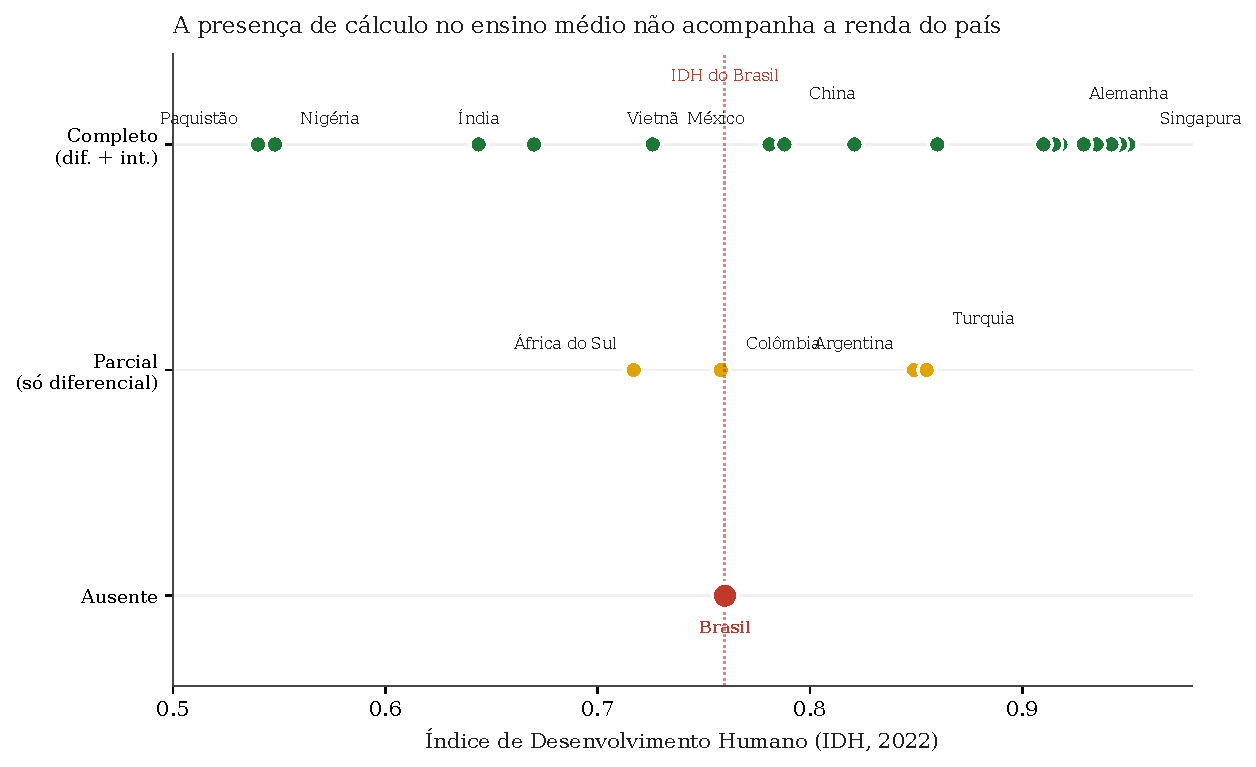
\includegraphics[width=0.95\textwidth]{fig03_hdi_calculo.pdf}
\caption{Índice de Desenvolvimento Humano (2022) versus presença de
cálculo no ensino médio. Cada ponto é um sistema nacional; o Brasil
(vermelho) é o único país que exclui simultaneamente o cálculo
diferencial e o integral, em qualquer faixa de IDH.}
\label{fig:hdi}
\end{figure}

\subsection{Síntese quantitativa}

O Quadro~\ref{quad:comparativo} sintetiza a presença de cálculo no ensino
médio dos sistemas de alta renda analisados, com o respectivo exame ou
sistema de admissão e o desempenho médio em matemática no PISA 2022,
quando disponível.

\begin{table}[H]
\centering
\caption{Cálculo no ensino médio em sistemas de alta renda: síntese}
\label{quad:comparativo}
\small
\begin{tabular}{@{}lllr@{}}
\toprule
\textbf{País / Sistema} & \textbf{Cálculo no EM} & \textbf{Exame / admissão} & \textbf{PISA 2022} \\
\midrule
Singapura       & H2 Math (sim)            & GCE A-Level         & 575 \\
Japão           & Math III (eletivo/STEM)  & EJU / vestibular    & 536 \\
Coreia do Sul   & Cálculo (eletivo)        & Suneung (CSAT)      & 527 \\
Finlândia       & Matemática longa         & Matrícula nacional  & 484 \\
Rússia          & EGE Profile              & EGE                 & 478 \\
Alemanha        & Analysis (obrigatório)   & Abitur              & 475 \\
França          & Spécialité Maths         & Baccalauréat        & 474 \\
Reino Unido     & A-Level Maths            & A-Level             & 489 \\
Canadá (Ontário)& Calculus and Vectors     & admissão provincial & 497 \\
Austrália       & Methods / Specialist     & admissão estadual   & 487 \\
Itália          & Liceo Scientifico (obr.) & Esame di Stato      & 471 \\
Espanha         & Matemáticas II           & EBAU/PAU            & 473 \\
Israel          & 5 unidades               & Bagrut              & 458 \\
Estados Unidos  & AP Calculus (eletivo)    & SAT/AP              & 465 \\
IB              & AA HL (sim)              & Diploma IB          & --- \\
\textbf{Brasil} & \textbf{Não}             & ENEM/vestibular     & \textbf{379} \\
\bottomrule
\end{tabular}
\fonte{Elaboração própria, a partir dos documentos curriculares oficiais
citados e de OECD (2023).}
\end{table}

A Figura~\ref{fig:heatmap} representa graficamente o contraste para um
subconjunto dos países, com o Brasil como única linha integralmente
ausente.

\begin{figure}[H]
\centering
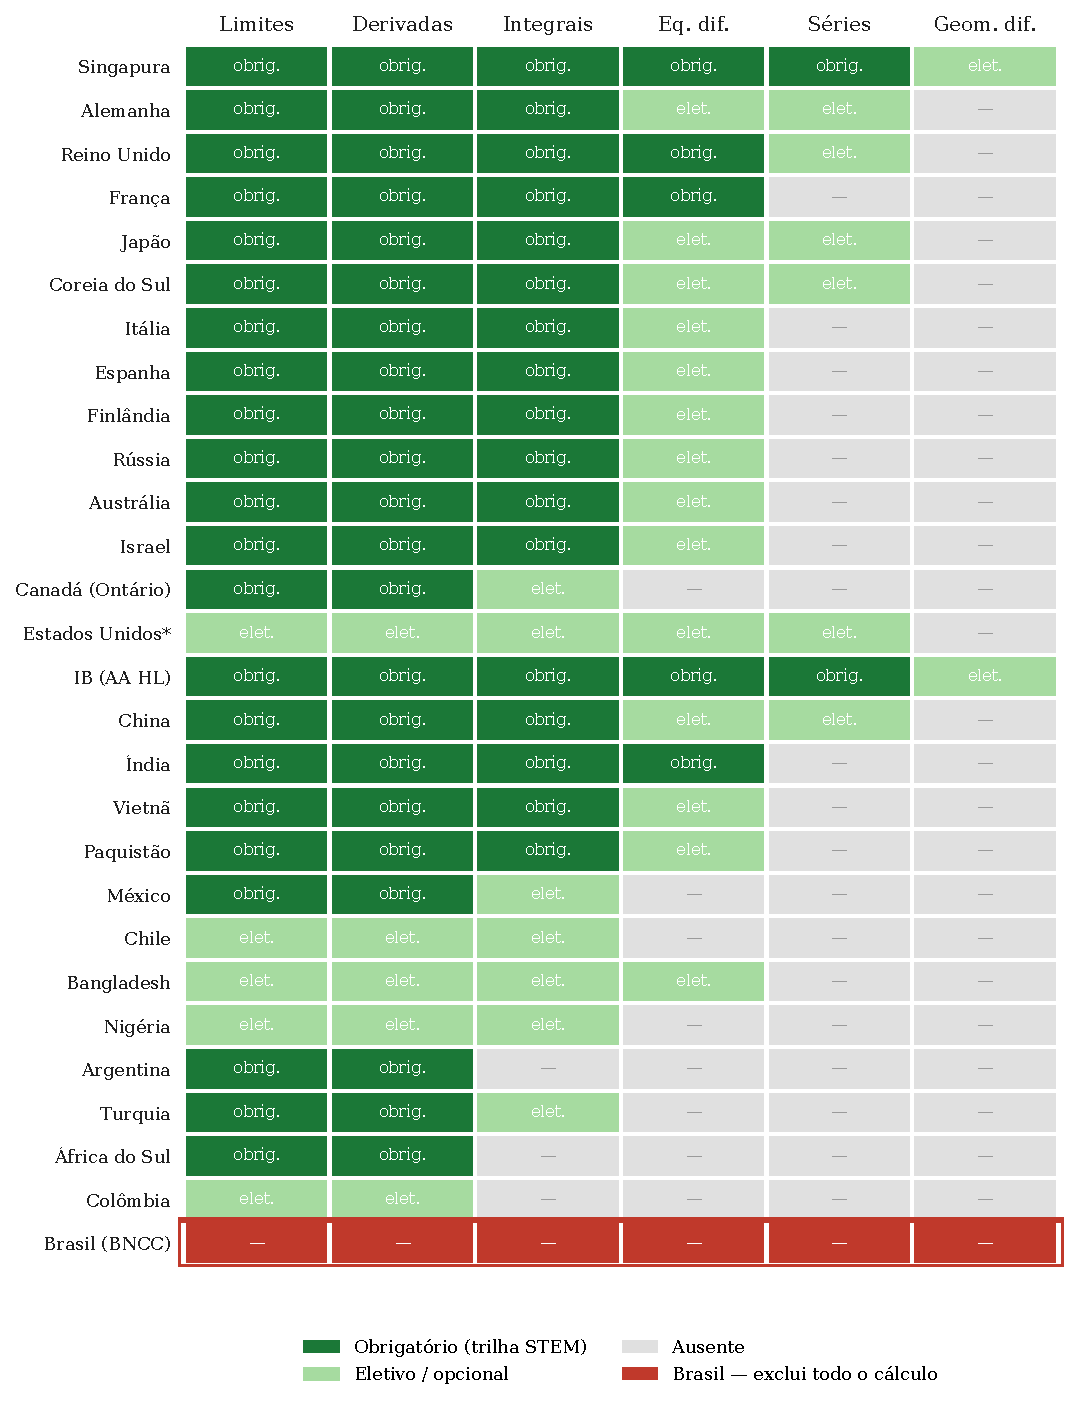
\includegraphics[width=0.74\textwidth]{fig01_heatmap_calculo.pdf}
\caption{Cálculo no ensino médio em 27 sistemas nacionais e no programa IB.
Cada célula indica se o tópico (limites, derivadas, integrais, equações
diferenciais, séries, geometria diferencial) é obrigatório, eletivo ou
ausente no currículo nacional para ingresso em cursos STEM. O Brasil
(BNCC) é a única linha integralmente ausente.}
\label{fig:heatmap}
\end{figure}

\subsection{Comparativo por idade: o que se aprende em cada faixa etária}

Esta subseção responde à pergunta operacional: tomado um estudante
qualquer dos países comparados, em que idade ele encontra qual conteúdo?
A análise organiza-se por idade-alvo (15, 16 e 17 anos), correspondendo
aproximadamente ao 1.\textsuperscript{o}, 2.\textsuperscript{o} e
3.\textsuperscript{o} anos do ensino médio brasileiro
(Quadros~\ref{quad:idade16} e \ref{quad:idade17}).

\begin{table}[H]
\centering
\caption{Conteúdo típico aos 16 anos, por país}
\label{quad:idade16}
\small
\begin{tabular}{@{}lp{3.2cm}p{2.6cm}p{5.2cm}@{}}
\toprule
\textbf{País} & \textbf{Cálculo} & \textbf{Estatística} & \textbf{Etapa} \\
\midrule
Japão        & Cálculo elementar       & Inferência básica & Math II + Math B \\
China        & Derivadas e aplicações  & Distribuições     & 11.\textsuperscript{o} ano \\
Singapura    & Diferenciação           & Probabilidade     & H2 Math (início) \\
Alemanha     & Cálculo diferencial     & Distrib. binomial & Klasse 11 \\
França       & Derivada formal         & Var. aleatórias   & Première \\
Coreia do Sul& Limites e cálculo       & Probabilidade     & Matemática II \\
Brasil       & ---                     & Estat. descritiva & Análise combinatória \\
\bottomrule
\end{tabular}
\fonte{Elaboração própria, a partir dos documentos curriculares citados.}
\end{table}

Aos 16 anos, o distanciamento se abre: na maioria dos sistemas
comparados, o estudante já realiza cálculo diferencial em algum nível,
enquanto no Brasil o conteúdo é análise combinatória e geometria ---
relevantes, mas sem interface com o cálculo.

\begin{table}[H]
\centering
\caption{Conteúdo típico aos 17 anos, por país}
\label{quad:idade17}
\small
\begin{tabular}{@{}lp{3.4cm}p{2.6cm}p{5cm}@{}}
\toprule
\textbf{País} & \textbf{Cálculo} & \textbf{Estatística} & \textbf{Etapa} \\
\midrule
Japão        & Math III: integração       & ---             & Vestibular STEM \\
China        & Integral + TFC             & Distribuições   & Trilha avançada \\
Singapura    & Integração + EDOs          & Hipótese, regr. & H2 Math (final) \\
Alemanha     & Integral + EDO             & Estocástica     & Abitur \\
França       & Integral + EDO             & Lei Grd. Núm.   & Terminale \\
Itália       & Análise (der.\ + int.)     & ---             & Esame di Stato \\
Reino Unido  & Diferenc. + integração     & ---             & A-Level \\
Rússia       & Diferenc. + primitivas     & Sim             & EGE Profile \\
EUA          & AP Calculus AB/BC (elet.)  & AP Statistics   & 12.\textsuperscript{o} ano \\
Brasil       & ---                        & Estat. descr.   & Geom.\ analítica, polinômios \\
\bottomrule
\end{tabular}
\fonte{Elaboração própria, a partir dos documentos curriculares citados.}
\end{table}

Aos 17 anos, a divergência é completa: na maioria dos sistemas, o
estudante encerra o ensino médio tendo coberto o equivalente ao Cálculo~I
universitário brasileiro. No Brasil, a matemática do 3.\textsuperscript{o}
ano cobre tópicos de pré-cálculo (geometria analítica, polinômios) que
\emph{seriam} pré-requisitos do cálculo, sem nunca chegar a ele. Bruner
(1960) descreveu exatamente esse padrão como antipadrão pedagógico:
apresentar um conceito complexo em sua forma final, sem revisitas
progressivas, tende a produzir compreensão superficial e baixa
transferência.

\subsection{O caso brasileiro: duzentos anos de currículo}

O caso brasileiro só se compreende em sua trajetória histórica. Ao
contrário do que sugere o senso comum, a ausência do cálculo no ensino
médio não é ``natural'' nem ``definitiva'': resulta de decisões
curriculares sucessivas, algumas das quais incluíram o cálculo no
programa antes de removê-lo.

\subsubsection{Império: o Colégio Pedro II (1837)}

O Colégio Pedro II, criado por decreto imperial de 2 de dezembro de 1837,
foi a primeira instituição de ensino secundário organizada no Brasil,
resultante da reorganização do Seminário de São Joaquim (Brasil, 1837).
Seu currículo inicial, de orientação humanística e clássica, incluía
matemática elementar, mas \emph{não} contemplava cálculo diferencial e
integral.

\subsubsection{República: a Reforma Benjamin Constant (1890) e sua reversão}

Após a Proclamação da República, Benjamin Constant promulgou o Decreto
n.\textsuperscript{o} 981, de 8 de novembro de 1890, que reorganizou o
``Ginásio Nacional''. Inspirado na hierarquia das ciências de Auguste
Comte, o decreto previu, no 3.\textsuperscript{o} ano, ``geometria geral
e seu complemento algébrico'' e ``cálculo diferencial e integral,
limitado ao conhecimento das teorias rigorosamente indispensáveis ao
estudo da mecânica geral'' (Brasil, 1890). Foi a primeira inclusão formal
do cálculo no currículo do ensino secundário brasileiro. Como mostra
Silva (2023), o cálculo foi efetivamente excluído do programa do Colégio
Pedro II já em 1899, situação consolidada na revisão geral promovida pelo
Decreto n.\textsuperscript{o} 3.890, de 1.\textsuperscript{o} de janeiro
de 1901 (Reforma Epitácio Pessoa) (Brasil, 1901). Desde então, o cálculo
não retornou ao currículo oficial do ensino secundário/médio brasileiro.

A janela 1890--1901 (entrada e saída do cálculo no secundário brasileiro)
constitui uma descontinuidade institucional documentada em fontes
primárias, cuja remoção foi exógena ao desempenho dos estudantes ---
seguiu-se à morte prematura de Benjamin Constant, em janeiro de 1891, e
ao realinhamento político subsequente, e não a uma avaliação técnica de
ineficácia (Silva, 2023).

\subsubsection{Era Vargas: a Reforma Capanema (1942)}

O Decreto-Lei n.\textsuperscript{o} 4.244, de 9 de abril de 1942 (Lei
Orgânica do Ensino Secundário, ou Reforma Capanema), estabeleceu o ensino
secundário em dois ciclos, com os cursos Clássico e Científico no
2.\textsuperscript{o} ciclo (Brasil, 1942). Incorporando propostas de
Euclides Roxo, o programa de matemática do Científico, fixado pela
Portaria Ministerial n.\textsuperscript{o} 177, de 1943, \emph{incluía o
estudo das variações e das derivadas}, mas \emph{não} o cálculo integral
(Dassie, 2001). A reforma, portanto, manteve a derivada em caráter
algébrico restrito e não recuperou a integral perdida em 1899.

\subsubsection{O Movimento da Matemática Moderna (1960--1980)}

Na década de 1960, sob influência do \emph{School Mathematics Study
Group} norte-americano, instaurou-se no Brasil o Movimento da Matemática
Moderna (MMM), tendo Osvaldo Sangiorgi e o Grupo de Estudos do Ensino de
Matemática (GEEM) como principais disseminadores (Búrigo, 1989; Soares,
2001). O MMM enfatizou conceitos abstratos --- teoria de conjuntos,
estruturas algébricas --- em detrimento do cálculo e da geometria
clássica, representando, do ponto de vista da introdução do cálculo, um
recuo. O movimento foi posteriormente criticado por sua abstração
excessiva e abandonado nas décadas de 1980--1990, mas seu legado
permanece detectável nos livros didáticos e nos parâmetros curriculares
subsequentes.

\subsubsection{PCN, PCNEM e BNCC (1997--2018)}

Os Parâmetros Curriculares Nacionais (1997) e sua versão para o ensino
médio (2000) marcaram a entrada oficial de tópicos de estatística e
probabilidade no currículo. A Base Nacional Comum Curricular (BNCC),
homologada em 2018, organiza a área de Matemática e suas Tecnologias do
ensino médio por competências e habilidades --- e não pelas cinco
unidades temáticas que estruturam o ensino fundamental (Brasil, 2018).
A BNCC do ensino médio \emph{não} inclui limites, derivadas ou integrais,
e a estatística prevista é descritiva, não inferencial. A própria SBEM
reconhece o problema:

\begin{quote}
\small
``Alguns livros didáticos do Ensino Médio apresentam tópicos de Cálculo
Diferencial e Integral, como limite, derivada e integral, mas na maioria
das vezes não são ensinados sob o pretexto de serem difíceis e impróprios
a esse segmento da educação [\ldots]. Assim sendo, o Cálculo faz parte do
livro didático, mas não do currículo do Ensino Médio.'' (SBEM, 2007).
\end{quote}

O Novo Ensino Médio (Lei n.\textsuperscript{o} 13.415/2017, reformulada
pela Lei n.\textsuperscript{o} 14.945/2024) instituiu itinerários
formativos, entre eles ``Matemática e suas Tecnologias'', que
\emph{permitem}, mas não \emph{exigem}, a oferta de cálculo, sem que isso
o tenha incorporado ao currículo comum obrigatório (Brasil, 2017; BRASIL,
2024).

\subsection{Consequências mensuráveis}

\subsubsection{Desempenho no PISA (2003--2022)}

O Brasil melhorou modestamente entre 2003 e 2009 e estagnou em torno de
380 pontos em matemática desde então, mantendo-se cerca de 90 a 145
pontos abaixo da média da OECD ao longo do período (Tabela~\ref{tab:pisa};
OECD, 2023). Apenas 1\% dos jovens brasileiros qualificam-se como
\emph{top performers} em matemática, contra 41\% em Singapura e 9\% na
média da OECD (OECD, 2023). O baixo desempenho persiste mesmo na
comparação regional: como mostra a Figura~\ref{fig:pisa}, o Brasil figura
na base do grupo latino-americano, abaixo de Chile, Uruguai, México, Peru
e Colômbia, e em patamar próximo ao da Argentina.

\begin{table}[H]
\centering
\captionsetup{name=Tabela}
\caption{Desempenho do Brasil em matemática no PISA (2003--2022)}
\label{tab:pisa}
\normalsize
\begin{tabular}{@{}rrrr@{}}
\toprule
\textbf{Ciclo} & \textbf{Brasil} & \textbf{Média OECD} & \textbf{Diferença} \\
\midrule
2003 & 356 & 499 & $-$143 \\
2006 & 370 & 494 & $-$124 \\
2009 & 386 & 495 & $-$109 \\
2012 & 389 & 494 & $-$105 \\
2015 & 377 & 490 & $-$113 \\
2018 & 384 & 489 & $-$105 \\
2022 & 379 & 472 & $-$93  \\
\bottomrule
\end{tabular}
\fonte{Elaboração própria, a partir de OECD (2023).}
\end{table}

\begin{figure}[H]
\centering
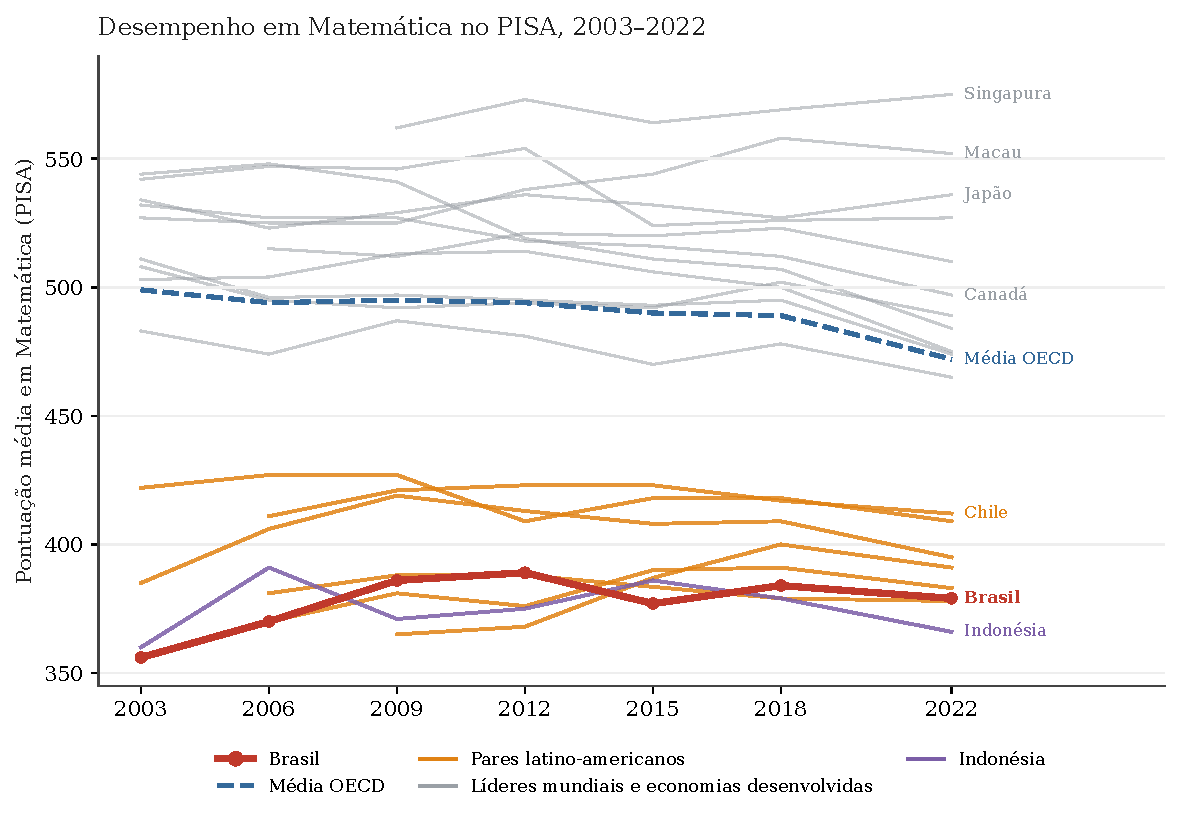
\includegraphics[width=0.95\textwidth]{fig02_pisa_timeline.pdf}
\caption{Desempenho em Matemática no PISA, 2003--2022, em vinte sistemas
educacionais. O Brasil (vermelho) oscila em torno de 380 pontos,
situando-se na base mesmo entre os pares latino-americanos (laranja); a
média da OECD (azul tracejada) e os líderes mundiais e economias
desenvolvidas (cinza) situam-se muito acima. O resultado da Argentina em
2015 foi omitido por incomparabilidade reconhecida pela OECD.}
\label{fig:pisa}
\end{figure}

Registre-se uma ressalva importante de identificação: o PISA avalia
estudantes de 15 anos, idade em que o cálculo ainda não foi introduzido
em \emph{nenhum} dos países da amostra. O desempenho brasileiro mede,
portanto, sobretudo a qualidade do ensino fundamental e condições
socioeconômicas, e não o efeito específico da ausência de cálculo no
ensino médio. Esse indicador é apresentado como contexto, não como
evidência do canal causal discutido na Seção~\ref{sec:discussao}.

\subsubsection{Reprovação em Cálculo~I}

A literatura é convergente quanto ao fato de o Cálculo~I ser, isoladamente,
a disciplina que mais reprova nas engenharias brasileiras, embora não
exista um índice nacional único e auditado. Estudos institucionais
reportam taxas elevadas e dispersas: cerca de 70\% na UFRJ (GAZETA DO
POVO, 2023); até 77,5\% de reprovação somada à evasão na Unicamp, entre
1997 e 2009 (Garzella, 2013); e ampla variação entre instituições em
revisões da literatura de educação em engenharia (Macambira; Athayde,
2014). A análise epistemológica de Rezende (2003) interpreta o fenômeno
como estrutural, e não conjuntural.

\subsubsection{O ``apagão de engenheiros''}

O CONFEA projeta déficit de até um milhão de profissionais das áreas
tecnológicas até 2030, associando-o à queda de matrículas e à fragilidade
da formação matemática de base (CONFEA, 2025). A causalidade entre
formação básica e déficit profissional não é direta nem única, mas a
literatura identifica o ciclo básico --- e o Cálculo~I em particular ---
como principal filtro de evasão nas engenharias.

\subsection{Exemplos comparativos: o que se cobra em cada exame?}

Para tornar concreta a discussão, apresentam-se exemplos típicos de
problemas de exames nacionais ao final do ensino médio. Os enunciados
estrangeiros exigem cálculo formal; o brasileiro, aritmética --- na mesma
faixa etária.

\smallskip
\noindent\fbox{\parbox{0.95\textwidth}{\small\textbf{Gaokao (China):}
Seja $f(x) = x^3 - 3ax + 2$. (1)~Discuta a monotonicidade de $f$.
(2)~Se $f$ tem mínimo igual a 0, determine $a$. (3)~Determine o número de
raízes reais de $f(x)=1$ em função de $a$.}}

\smallskip
\noindent\fbox{\parbox{0.95\textwidth}{\small\textbf{Abitur
Leistungskurs (Alemanha):} Seja $f(x) = x\,e^{-x^2}$. (a)~Determine e
classifique os pontos críticos. (b)~Calcule a área entre o gráfico de $f$
e o eixo $x$ para $x \geq 0$.}}

\smallskip
\noindent\fbox{\parbox{0.95\textwidth}{\small\textbf{AP Calculus BC
(EUA):} Determine o intervalo de convergência da série
$\sum_{n=1}^{\infty} \dfrac{(x-2)^n}{n\,3^n}$, justificando o teste
utilizado.}}

\smallskip
\noindent\fbox{\parbox{0.95\textwidth}{\small\textbf{ENEM (Brasil):} Em
um experimento, o número de bactérias dobra a cada hora. Se inicialmente
havia 100 bactérias, quantas haverá após 5 horas? (a)~500 (b)~1.000
(c)~1.600 (d)~3.200 (e)~6.400.}}

\smallskip
O ENEM cobra crescimento exponencial em forma discreta, sem interface com
a derivada da exponencial nem com a noção de taxa instantânea ---
contraste que ilustra, de modo tangível, o vácuo curricular documentado.

\subsection{Discussão: níveis de robustez e contra-argumentos}
\label{sec:discussao}

A análise permite distinguir três níveis de afirmação, com graus
distintos de robustez. \textbf{Nível 1 --- fato curricular}: o Brasil é o
único país da amostra cujo currículo nacional do ensino médio não inclui
cálculo (robustez alta). \textbf{Nível 2 --- correlações observadas}: o
Brasil tem desempenho substancialmente inferior em avaliações
internacionais e taxas elevadas de reprovação em Cálculo~I (robustez
alta). \textbf{Nível 3 --- inferência causal}: a ausência de cálculo no
ensino médio \emph{contribui} para esses indicadores (robustez moderada;
há fatores confundidores, como qualidade geral do ensino básico,
condições socioeconômicas e formação docente).

Em fidelidade ao princípio acadêmico de considerar os argumentos
contrários em sua versão mais forte, registram-se as principais objeções:
(C1)~``a base é fraca demais'' --- objeção parcialmente válida, mas
endereçável por sequenciamento em espiral; (C2)~``não há professores
qualificados'' --- objeção empiricamente forte, que demanda investimento
em formação docente; (C3)~``não cabe na carga horária'' --- a comparação
internacional mostra cargas semanais maiores em vários sistemas,
sugerindo reorganização de prioridades; e (C4)~``aumentaria a
desigualdade'' --- objeção politicamente relevante, mas tecnicamente
reversível, pois a estratificação \emph{já} existe (estudantes de IB em
escolas particulares brasileiras estudam cálculo, ao passo que a rede
pública não o oferece), de modo que incorporá-lo à BNCC tenderia a
\emph{reduzir} a desigualdade.

% =====================================================================
% 5. CONSIDERAÇÕES FINAIS
% =====================================================================
\section{Considerações Finais}

Este artigo documentou, com base em fontes curriculares oficiais de
sistemas educacionais de cinco continentes, que o Brasil é o único da
amostra cujo currículo nacional do ensino médio não inclui cálculo
diferencial e integral. O fato é verificável e historicamente conhecido:
em duzentos anos de trajetória educacional, o cálculo esteve presente no
secundário brasileiro apenas em um período breve --- entre a Reforma
Benjamin Constant (1890) e sua reversão (1899--1901) ---, com a derivada
brevemente recuperada, em caráter restrito, pela Reforma Capanema (1942).

O arcabouço pedagógico que tornaria viável a reintrodução está
consolidado --- o currículo em espiral de Bruner, a zona de
desenvolvimento proximal de Vygotsky e o diagnóstico epistemológico de
Rezende ---, e o caso de Singapura evidencia, em escala nacional, que sua
aplicação sistemática produz resultados. A inferência causal estrita
entre o vácuo curricular e os indicadores mensuráveis permanece difícil
de estabelecer; a correlação, contudo, é robusta, e a literatura
brasileira converge, desde Ávila (1991), para a hipótese de que a
intervenção curricular seria parte da solução.

Mais do que prescrever uma reforma --- tarefa de longa maturação política
e técnica ---, o artigo pretende oferecer um mapeamento preciso e
replicável de um contraste internacional pouco quantificado na literatura
nacional. Pesquisas futuras poderão (i) ampliar a amostra de países de
renda média e baixa; (ii) realizar análise de séries temporais
interrompidas sobre coortes históricas de ingresso em engenharia; e
(iii) desenhar e avaliar experimentalmente sequências didáticas de
introdução ao cálculo no ensino médio brasileiro. O Brasil é exceção
curricular; não precisa continuar sendo.

% ---------- AGRADECIMENTOS / DECLARAÇÕES (anonimizadas) --------------
\section*{Agradecimentos}
\textit{[Suprimido para avaliação por pares duplo-cega. Será inserido na
versão final, conforme política da revista.]}

\section*{Declarações}
\noindent\textbf{Conflito de interesse.} Os autores declaram não haver
conflito de interesse. \textbf{Financiamento.} A pesquisa não recebeu
financiamento externo. \textbf{Contribuição.} Todos os autores
contribuíram para a concepção do estudo, a curadoria das fontes e a
redação, tendo aprovado a versão submetida.

% =====================================================================
% REFERÊNCIAS  (ABNT NBR 6023; chamadas autor-data NBR 10520:2023)
% =====================================================================
\newpage
\section*{Referências}
\addcontentsline{toc}{section}{Referências}

\begingroup
\setstretch{1.0}
\setlength{\parindent}{0pt}
\raggedright
\newcommand{\refitem}[1]{\par #1\par\vspace{12pt}}

\refitem{ÁFRICA DO SUL. Department of Basic Education. \textbf{Curriculum
and Assessment Policy Statement (CAPS), FET Phase, Grades 10--12:
Mathematics}. Pretória: DBE, 2011.}

\refitem{ALEMANHA. Kultusministerkonferenz (KMK). \textbf{Bildungsstandards
im Fach Mathematik für die Allgemeine Hochschulreife}. Berlim: KMK, 2012.
Disponível em:
\url{https://www.kmk.org/fileadmin/veroeffentlichungen_beschluesse/2012/2012_10_18-Bildungsstandards-Mathe-Abi.pdf}.
Acesso em: 6 jun. 2026.}

\refitem{ARGENTINA. Dirección General de Cultura y Educación (Provincia
de Buenos Aires). \textbf{Diseño Curricular para la Educación Secundaria
--- Matemática, Ciclo Superior, 6.\textsuperscript{o} año}. La Plata:
DGCyE, 2011.}

\refitem{AUSTRÁLIA. Australian Curriculum, Assessment and Reporting
Authority (ACARA). \textbf{The Australian Curriculum: Senior Secondary ---
Mathematics} (v.~8.4). Sydney: ACARA, 2015. Disponível em:
\url{https://www.australiancurriculum.edu.au/senior-secondary-curriculum/mathematics/}.
Acesso em: 6 jun. 2026.}

\refitem{ÁVILA, Geraldo. O ensino de Cálculo no 2.\textsuperscript{o}
grau. \textbf{Revista do Professor de Matemática}, Rio de Janeiro, n. 18,
p. 1--9, 1991.}

\refitem{BANGLADESH. National Curriculum and Textbook Board (NCTB).
\textbf{Higher Secondary (XI--XII) Higher Mathematics Syllabus}. Daca:
NCTB, 2022.}

\refitem{BRASIL. \textbf{Decreto de 2 de dezembro de 1837}. Cria o
Colégio de instrução secundária (Colégio Pedro II). Rio de Janeiro, 1837.}

\refitem{BRASIL. \textbf{Decreto n.\textsuperscript{o} 981, de 8 de
novembro de 1890}. Aprova o Regulamento da Instrução Primária e Secundária
do Distrito Federal (Reforma Benjamin Constant). Rio de Janeiro, 1890.}

\refitem{BRASIL. \textbf{Decreto n.\textsuperscript{o} 3.890, de
1.\textsuperscript{o} de janeiro de 1901}. Código dos Institutos Oficiais
de Ensino Superior e Secundário (Reforma Epitácio Pessoa). Rio de
Janeiro, 1901.}

\refitem{BRASIL. \textbf{Decreto-Lei n.\textsuperscript{o} 4.244, de 9 de
abril de 1942}. Lei Orgânica do Ensino Secundário (Reforma Capanema). Rio
de Janeiro, 1942.}

\refitem{BRASIL. \textbf{Lei n.\textsuperscript{o} 13.415, de 16 de
fevereiro de 2017}. Altera as Leis de Diretrizes e Bases e institui a
Política de Fomento ao Ensino Médio em Tempo Integral. Brasília, 2017.}

\refitem{BRASIL. Ministério da Educação. \textbf{Base Nacional Comum
Curricular}. Brasília: MEC, 2018.}

\refitem{BRASIL. \textbf{Lei n.\textsuperscript{o} 14.945, de 31 de julho
de 2024}. Altera a Lei n.\textsuperscript{o} 9.394/1996 quanto à
organização do ensino médio. Brasília, 2024.}

\refitem{BRUNER, Jerome S. \textbf{The process of education}. Cambridge,
MA: Harvard University Press, 1960.}

\refitem{BRUNER, Jerome S. \textbf{Toward a theory of instruction}.
Cambridge, MA: Belknap Press of Harvard University Press, 1966.}

\refitem{BÚRIGO, Elisabete Zardo. \textbf{Movimento da Matemática Moderna
no Brasil}: estudo da ação e do pensamento de educadores matemáticos nos
anos 60. 1989. Dissertação (Mestrado em Educação) --- Universidade Federal
do Rio Grande do Sul, Porto Alegre, 1989.}

\refitem{CANADÁ. Ministry of Education (Ontario). \textbf{The Ontario
Curriculum, Grades 11 and 12: Mathematics} (revised). Toronto: Queen's
Printer for Ontario, 2007. Disponível em:
\url{https://www.edu.gov.on.ca/eng/curriculum/secondary/math1112currb.pdf}.
Acesso em: 6 jun. 2026.}

\refitem{CAPELATO, Erika; ZUBIRÍAS, Gabriela Cervantes. Intercâmbio
virtual no ensino superior: limitações e potencialidades para o ensino e
aprendizagem de Cálculo. \textbf{Revista de Educação Matemática}, São
Paulo, v. 24, 2025. Disponível em:
\url{https://www.revistasbemsp.com.br/index.php/REMat-SP/article/view/710}.
Acesso em: 6 jun. 2026.}

\refitem{CBSE --- Central Board of Secondary Education.
\textbf{Mathematics (041) Syllabus, Classes XI--XII (2023--24)}. Nova
Délhi: CBSE, 2023.}

\refitem{CHILE. Ministerio de Educación (Unidad de Currículum y
Evaluación). \textbf{Programa de Estudio 3.\textsuperscript{o} o
4.\textsuperscript{o} Medio, Formación Diferenciada --- Matemática:
Límites, Derivadas e Integrales}. Santiago: MINEDUC, 2021.}

\refitem{CHINA. Ministério da Educação. \textbf{Currículo nacional de
matemática do ensino médio} [Pu tong gao zhong shu xue ke cheng biao
zhun], ed. 2017, rev. 2020. Pequim: People's Education Press, 2020.}

\refitem{COLLEGE BOARD. \textbf{AP Calculus AB and AP Calculus BC course
and exam description}. Nova York: College Board, 2020. Disponível em:
\url{https://apcentral.collegeboard.org/media/pdf/ap-calculus-ab-and-bc-course-and-exam-description.pdf}.
Acesso em: 6 jun. 2026.}

\refitem{COLÔMBIA. Ministerio de Educación Nacional. \textbf{Estándares
Básicos de Competencias en Matemáticas}. Bogotá: MEN, 2006.}

\refitem{CONFEA. \textbf{Confea alerta para déficit de engenheiros e
defende foco na matemática}. Brasília: Conselho Federal de Engenharia e
Agronomia, 2025. Disponível em:
\url{https://www.confea.org.br/confea-alerta-para-deficit-de-engenheiros-e-defende-foco-na-matematica}.
Acesso em: 6 jun. 2026.}

\refitem{COREIA DO SUL. Ministry of Education. \textbf{Mathematics
Curriculum} (Notification n. 2015-74, Annex 8). Sejong: Ministry of
Education, 2015.}

\refitem{DALTO, Jader Otavio; SILVA, Karina Alessandra Pessoa da;
BORSSOI, Adriana Helena. Práticas avaliativas em uma disciplina de
Cálculo Diferencial e Integral no contexto remoto: aspectos evidenciados.
\textbf{Revista de Educação Matemática}, São Paulo, v. 19, n. esp.,
e022038, 2022.}

\refitem{DASSIE, Bruno Alves. \textbf{A matemática do curso secundário na
Reforma Gustavo Capanema}. 2001. Dissertação (Mestrado) --- Pontifícia
Universidade Católica do Rio de Janeiro, Rio de Janeiro, 2001.}

\refitem{ESPANHA. Ministerio de Educación y Formación Profesional.
\textbf{Real Decreto 243/2022}, de 5 de abril, por el que se establecen
la ordenación y las enseñanzas mínimas del Bachillerato. Boletín Oficial
del Estado, Madrid, n. 82, 6 abr. 2022.}

\refitem{FINLÂNDIA. Finnish National Agency for Education (EDUFI).
\textbf{National core curriculum for general upper secondary education
2019}. Helsinki: EDUFI, 2019.}

\refitem{FRANÇA. Ministère de l'Éducation Nationale et de la Jeunesse.
\textbf{Programme de spécialité de mathématiques de la classe terminale
de la voie générale}. Bulletin officiel spécial n. 1, 22 jan. 2019.
Paris: MENJ, 2019.}

\refitem{GARZELLA, Fabiana Colombo. \textbf{A disciplina de Cálculo I}:
análise das relações entre as práticas pedagógicas do professor e seus
impactos nos alunos. 2013. Tese (Doutorado em Educação) --- Universidade
Estadual de Campinas, Campinas, 2013.}

\refitem{GAZETA DO POVO. \textbf{UFRJ vai mudar currículo de cálculo para
tentar evitar evasão}. Curitiba, 2023.}

\refitem{INTERNATIONAL BACCALAUREATE ORGANIZATION (IBO). \textbf{Diploma
Programme --- Mathematics: Analysis and Approaches guide} (first
assessment 2021). Cardiff: IBO, 2019.}

\refitem{ITÁLIA. Ministero dell'Istruzione, dell'Università e della
Ricerca. \textbf{Indicazioni nazionali riguardanti gli obiettivi
specifici di apprendimento per i percorsi liceali}. Decreto
Interministeriale n. 211, 7 ott. 2010. Roma: MIUR, 2010.}

\refitem{JAPAN STUDENT SERVICES ORGANIZATION (JASSO). \textbf{EJU syllabus
for mathematics}. Tóquio: JASSO, 2025. Disponível em:
\url{https://www.jasso.go.jp/en/ryugaku/eju/examinee/syllabus/mathematics.html}.
Acesso em: 6 jun. 2026.}

\refitem{KONTOROVICH, Igor'. Research as a resource in a high-school
calculus curriculum. \textbf{ZDM --- Mathematics Education}, v. 53, p.
429--440, 2021. DOI: 10.1007/s11858-021-01236-3.}

\refitem{LEONG, Yew Hoong; HO, Weng Kin; CHENG, Lu Pien.
Concrete-Pictorial-Abstract: surveying its origins and charting its
future. \textbf{The Mathematics Educator}, Singapura, v. 16, n. 1, p.
1--19, 2015.}

\refitem{MACAMBIRA, Indira Quaresma; ATHAYDE, Lígia S. Reprovação na
disciplina cálculo nos cursos de engenharia: análise de dados e métodos
minimizadores. \emph{In}: CONGRESSO BRASILEIRO DE EDUCAÇÃO EM ENGENHARIA
(COBENGE), 42., 2014. \textbf{Anais [\ldots]}. Brasília: ABENGE, 2014.}

\refitem{MÉXICO. Secretaría de Educación Pública (DGB/SEMS). \textbf{Marco
Curricular Común de la Educación Media Superior --- Pensamiento
Matemático}. Cidade do México: SEP, 2023.}

\refitem{MULLIS, Ina V. S. \emph{et al.} \textbf{TIMSS 2015 international
results in mathematics}. Chestnut Hill, MA: TIMSS \& PIRLS International
Study Center, Boston College, 2016.}

\refitem{OECD. \textbf{PISA 2022 results (Volume I)}: the state of
learning and equity in education. Paris: OECD Publishing, 2023.}

\refitem{PAQUISTÃO. Federal Board of Intermediate and Secondary Education
(FBISE). \textbf{Scheme of Studies --- Mathematics HSSC-II}. Islamabad:
FBISE, 2023.}

\refitem{PNUD --- Programa das Nações Unidas para o Desenvolvimento.
\textbf{Relatório de Desenvolvimento Humano 2023/2024}. Nova York: PNUD,
2024.}

\refitem{REINO UNIDO. Department for Education. \textbf{Mathematics: AS
and A level content}. Londres: DfE, 2016. Ref. DFE-00706-2014.}

\refitem{REZENDE, Wanderley Moura. \textbf{O ensino de Cálculo}:
dificuldades de natureza epistemológica. 2003. Tese (Doutorado em
Educação) --- Faculdade de Educação, Universidade de São Paulo, São Paulo,
2003.}

\refitem{RÚSSIA. Federal Institute of Pedagogical Measurements (FIPI).
\textbf{Exame Estatal Unificado (EGE) --- Matemática, nível Profile}:
codificador de conteúdos. Moscou: FIPI, 2024.}

\refitem{SEAB --- Singapore Examinations and Assessment Board.
\textbf{Mathematics: Singapore-Cambridge GCE A-Level Higher 2 (Syllabus
9758)}. Singapura: SEAB; Ministry of Education, 2025.}

\refitem{SILVA, Circe Mary Silva da. Positivismo, ensino secundário e
cálculo diferencial e integral. \textbf{Revista História da Educação},
v. 27, e128201, 2023. DOI: 10.1590/2236-3459/128201.}

\refitem{SOARES, Flávia. \textbf{Movimento da Matemática Moderna no
Brasil}: avanço ou retrocesso? 2001. Dissertação (Mestrado) --- Pontifícia
Universidade Católica do Rio de Janeiro, Rio de Janeiro, 2001.}

\refitem{SOCIEDADE BRASILEIRA DE EDUCAÇÃO MATEMÁTICA (SBEM). O Cálculo
Diferencial e Integral e o Ensino Médio. \emph{In}: ENCONTRO NACIONAL DE
EDUCAÇÃO MATEMÁTICA (ENEM), 9., 2007, Belo Horizonte. \textbf{Anais
[\ldots]}. Recife: SBEM, 2007.}

\refitem{TEIXEIRA, Alessandra Carvalho. O Novo Ensino Médio e as
prescrições curriculares de Matemática para o estado de São Paulo em
2024. \textbf{Revista de Educação Matemática}, São Paulo, v. 21, 2024.
DOI: 10.37001/remat25269062v21id518.}

\refitem{TURQUIA. Millî Eğitim Bakanlığı (MEB). \textbf{Ortaöğretim
Matematik Dersi Öğretim Programı}. Ancara: MEB, 2018.}

\refitem{VIETNÃ. Bo Giao duc va Dao tao (MOET). \textbf{Chuong trinh Giao
duc Pho thong mon Toan} (Circular 32/2018/TT-BGDDT). Hanói: MOET, 2018.}

\refitem{VYGOTSKY, Lev S. \textbf{Mind in society}: the development of
higher psychological processes. Cambridge, MA: Harvard University Press,
1978.}

\refitem{WAEC --- West African Examinations Council. \textbf{Further
Mathematics Syllabus (WASSCE/SSCE)}. Lagos: WAEC, 2023.}

\refitem{WOOD, David; BRUNER, Jerome S.; ROSS, Gail. The role of tutoring
in problem solving. \textbf{Journal of Child Psychology and Psychiatry},
v. 17, n. 2, p. 89--100, 1976.}

\endgroup

\end{document}
